\renewcommand{\figurename}{Rys.}

\chapter{Właściwości optyczne tkanek}
\label{cha:WlasciowosciOptyczne}

\fontsize{14}{15}\selectfont
%---------------------------------------------------------------------------

Selektywne właściwości optyczne tkanek umożliwiają określanie istotnych cech zbiorów komórek przy zastosowaniu
optoelektronicznych metod pomiarowych, szczególnie przydatnych w~diagnostyce nieinwazyjnej. Wśród stosowanych sposobów 
pomiaru parametrów tkanek, wyróżnia się tendencja do rozwoju metod bazujących na detekcji i~analizie naturalnych oraz wymuszonych 
zjawisk biooptycznych~\cite{Cys:2007}.

Badany obiekt biologiczny jest jednorodną lub złożoną mieszaniną ciał stałych, cieczy i~gazów. Wewnątrz struktury tkankowej,
jak i~na granicy poszczególnych warstw komórek, zachodzą złożone zjawiska optyczne~(rys.~\ref{rys:light_interaction}), z~których 
najbardziej istotne to odbicie, refrakcja, absorpcja oraz rozpraszanie~\cite{Valisue:Thesis:2011}. Ich intensywność zależy od grubości, 
stopnia niejednorodności i~indywidualnych cech optycznych badanego obiektu.

\section{Refrakcja i~odbicie promieniowania}
\label{sec:refraction}
%---------------------------------------------------------------------------

Są to zjawiska optyczne występujące wyłącznie na granicy dwóch mediów transmisyjnych o~różnych współczynnikach refrakcji $n$. Załamanie (refrakcja) wiązki promieniowania
związane jest ze zmianą prędkości propagacji fali na skutek przejścia do ośrodka o~odmiennych właściwościach optycznych. Zjawisko refrakcji opisuje prawo Snella~\cite{Feyn:2012} 
w~postaci:

\begin{equation}
	v_{i}sin(\theta_{i})=v_{t}sin(\theta_{t})
\end{equation}
gdzie $\theta_{i}$ jest kątem padania promieniowania, $\theta_{t}$ kątem załamania, a~$v_{i}$ oraz $v_{t}$ są prędkościami propagacji fali 
wewnątrz ośrodków, które ze współczynnikami refrakcji łączy zależność $n=\frac{c}{v}$~\cite{Feyn:2012},~(c - prędkość światła w~próżni).\\

\begin{figure}[ht]
	\centerline{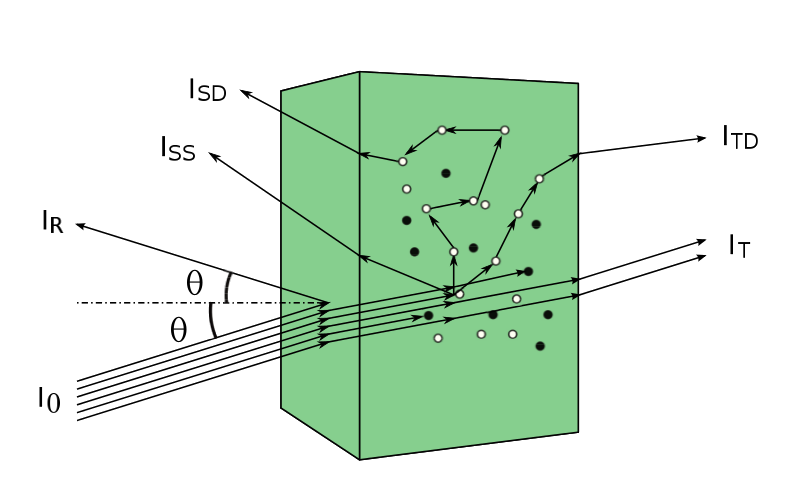
\includegraphics[scale = 0.50]{graphic/light_interaction.png}}
	\caption{Interakcja promieniowania elektromagnetycznego z~materią. Natężenie wejściowe światła~($I_{0}$), odbite~($I_{R}$), 
	rozproszone wstecz ($I_{SS}$, $I_{SD}$), wyjściowe ($I_{TD}$, $I_{T}$)}
	~\\	
	(źródło: Na podstawie \cite{Valisue:Thesis:2011})
	\label{rys:light_interaction}
\end{figure}
Zmiana kierunku rozchodzenia się fali na granicy dwóch ośrodków, powodująca, że pozostaje ona w~ośrodku, w~którym się rozchodzi definiuje prawo 
odbicia~\cite{Feyn:2012}. Kąt odbicia jest równy kątowi padania, a~promień padający, promień odbity i~normalna do powierzchni odbicia leżą w~jednej 
płaszczyźnie~(rys.~\ref{rys:refraction}). W~wyniku odbicia zmienia się tylko kierunek rozchodzenia się fali, nie zmienia się jej długość.

\begin{figure}[ht]
	\centerline{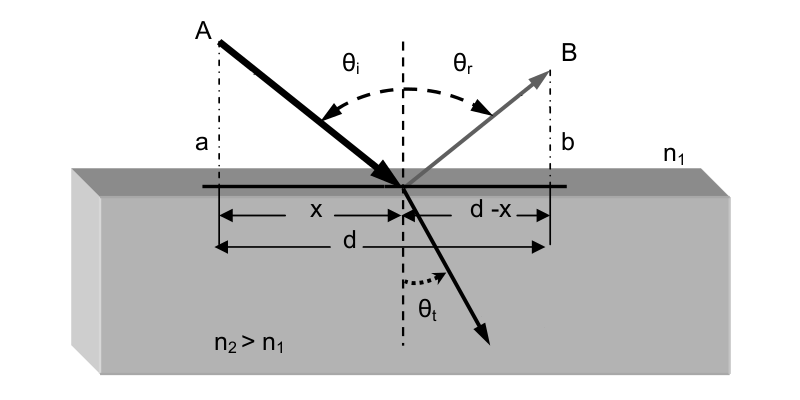
\includegraphics[scale = 0.53]{graphic/refraction.png}}
	\caption{Załamanie i~odbicie promieniowania elektromagnetycznego na granicy dwóch ośrodków o~współczynnikach refrakcji $n_{1}$~i~$n_{2}$}
	~\\
	(źródło: Na podstawie \cite{Yavari:PhD:2006})
	\label{rys:refraction}
\end{figure}


\section{Absorpcja}
\label{sec:Absorpcja}
%---------------------------------------------------------------------------

Natężenie wiązki promieniowania elektromagnetycznego jest redukowane w~miarę przenikania przez ośrodek materialny na skutek 
oddziaływania z~materią. Pochłonięta część energii promieniowania pierwotnego przechodzi przy tym w~inne formy energii (energia wewnętrzna ośrodka, 
energia wzbudzenia lub jonizacji, energia wtórnego promieniowania elektromagnetycznego)~\cite{Feyn:2012}.

Z~mikroskopowego punktu widzenia oraz według zasad fizyki kwantowej, poziomy energetyczne atomów i~cząsteczek są skwantyzowane~\cite{Yavari:PhD:2006}.
W~procesie absorpcji światło zachowuje się jak strumień cząstek elementarnych i~może być pochłaniane tylko w~określonych porcjach energii $E$, których 
wielkość zależy od częstotliwości $\nu$~(\ref{equ:planc}):

\begin{equation}
	E = h\nu
\label{equ:planc}
\end{equation}
$h$ - stała Plancka.\\

Kwant światła, czyli foton niosący określoną porcję energii może oddziaływać z~elektronem walencyjnym w~atomie substancji ośrodka. Jeżeli 
energia fotonu równa jest różnicy energii pomiędzy dowolnym stanem wzbudzonym elektronu a~stanem podstawowym, wówczas foton zostanie pochłonięty 
(rys.~\ref{rys:absorption}). 
Gdy energia fotonu jest inna, wówczas albo przechodzi on przez substancję bez przeszkód, albo jest rozpraszany. Na skutek absorpcji fotonu elektron 
przechodzi w~stan wzbudzenia o~wyższej energii~\cite{Yavari:PhD:2006}.

\begin{figure}[ht]
	\centerline{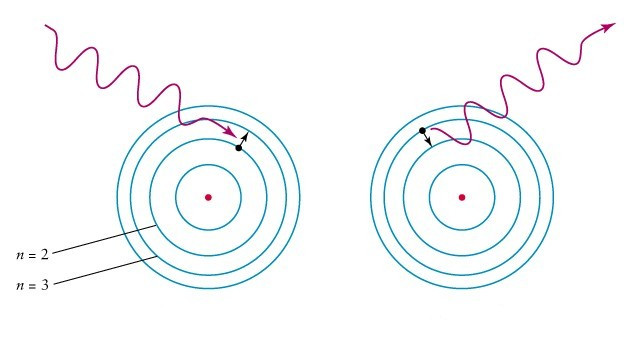
\includegraphics[scale = 0.62]{graphic/absorption.jpg}}
	\caption{Absorpcja spontaniczna. Elektron pochłania energię fotonu, dzięki czemu następuje wzbudzenie go na wyższy poziom energetyczny. Emisja 
	 	 to zjawisko odwrotne do absorpcji}
	~\\
	(źródło: http://www.candela.strefa.pl) 
	\label{rys:absorption}
\end{figure}

\subsection{Prawo Lamberta-Bouguera}
\label{subsec:LambertBouguer}
%---------------------------------------------------------------------------
Prawo Lamberta-Bouguera ilościowo opisuje proces absorpcji światła przez roztwory substancji barwnych podczas przenikania promieniowania 
monochromatycznego przez roztwór. Zależność opisująca stopień pochłaniania promieniowania w~stosunku do grubości ośrodka absorbującego po raz 
pierwszy podana została przez Bouguera w~1729 roku w~następującej postaci~\cite{Yavari:PhD:2006}:

\begin{equation}
	\frac{dI}{I} = \mu_{a}(\lambda)dx
	\label{equ:LambertBouguer}
\end{equation}
gdzie:\\
$x$ - grubość warstwy ośrodka,\\
$I$ - natężenie światła padającego,\\
$\mu_{a}(\lambda)$ - współczynnik absorpcji światła.\\\\
Rozwiązanie równania~(\ref{equ:LambertBouguer}) względem $x$ pokazuje, iż wartość promieniowania przenikającego przez roztwór maleje wykładniczo 
wraz z~grubością ośrodka~(rys.~\ref{rys:bouguer}). W~odlegości $x$ od powierzchni nadawczej w~ośrodku o~współczynniku pochłaniania $\mu_{a}(\lambda)$ wynosi:

\begin{equation}
	I(x) = Ie^{-\mu_{a}(\lambda) x}
\end{equation}
gdzie:\\
$I(x)$ - natężenie światła po przejściu przez warstwę ośrodka o~grubości~$x$\\
$e$ - podstawa logarytmu naturalnego.\\

\begin{figure}[ht]
	\centerline{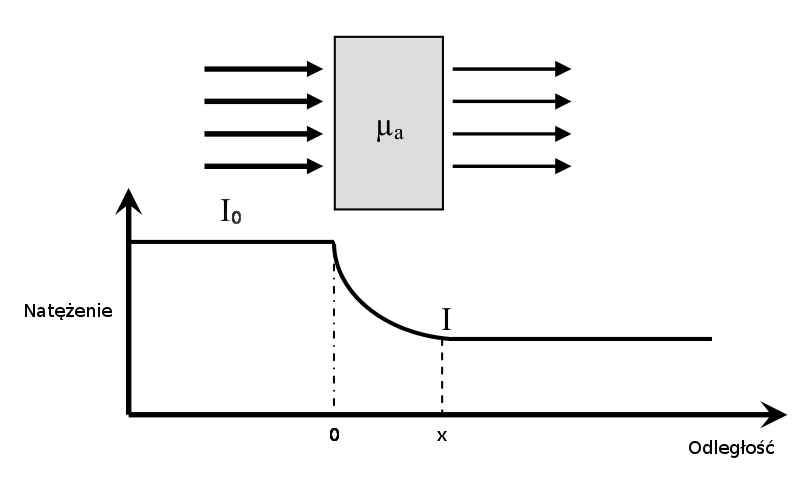
\includegraphics[scale = 0.5]{graphic/bouguer.png}}
	\caption{Absorpcja promieniowania w~jednorodnym ośrodku pochłaniającym o~współczynniku absorpcji $\mu_{a}$}
	~\\
	(źródło: Na podstawie \cite{Yavari:PhD:2006})
	\label{rys:bouguer}
\end{figure}

\subsection{Prawo Lamberta-Beera}
\label{subsec:BeerLambert}

W~1852 roku na bazie prowadzonych doświadczeń dowiedziono, iż wartość współczynnika absorpcji $\mu_{a}(\lambda)$ dla określonej długości fali jest wprost 
proporcjonalna do stężenia substancji absorbującej~\cite{Yavari:PhD:2006}.\\

\begin{equation}
	\mu_{a}(\lambda) = c\alpha(\lambda)
\end{equation}
gdzie:\\
$c$ - stężenie molowe substancji absorbującej w~roztworze,\\
$\alpha(\lambda)$ - molowy współczynnik absorpcji zwany absorbancją molową.

\noindent Zestawiając prawo Lamberta-Bouguera z~prawem Lamberta-Beera otrzymano kompletny opis zjawiska absorpcji promieniowania w~ośrodku absorbującym w~postaci:

\begin{equation}
	I(x) = Ie^{(-c\alpha(\lambda) x)}\\
\end{equation}
 
\begin{figure}[ht]
	\centerline{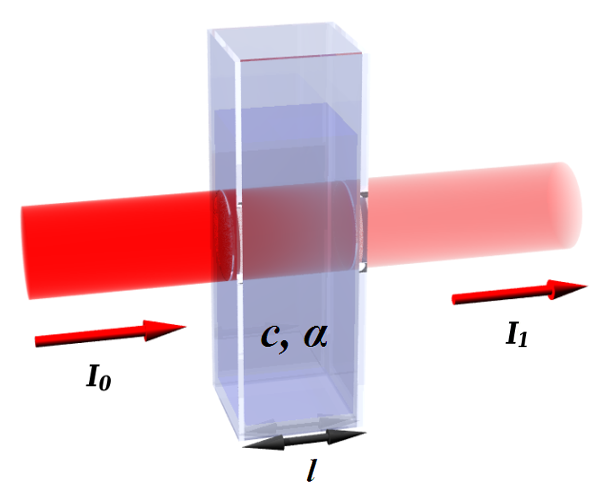
\includegraphics[scale = 0.44]{graphic/Beer_lambert.png}}
	\caption{Absorpcja światła przechodzącego przez substancję o~stężeniu molowym $c$ i~molowym współczynniku absorpcji $\alpha(\lambda)$}
	~\\
	(źródło: http://pl.wikipedia.org)
	\label{rys:Beer_lambert}
\end{figure}


\subsubsection{Prawo addytywności absorpcji}
\label{subsub:add}

W~przypadku roztworów złożonych z~wielu substancji o~różnych właściwościach optycznych, matematyczna reprezentacja prawa Lamberta-Beera jest superpozycją 
absorpcji każdego składnika z~osobna~\cite{Yavari:PhD:2006}:  
\begin{equation}
	I(x) = Ie^{-A}
	\label{equ:multilayer1}
\end{equation}
Dla środowiska niejednorodnego~(rys.~\ref{rys:multilayer}) absorbancja $A$ określana jest według zależności:
\begin{equation}
	A=c_{1}\alpha_{1}(\lambda)x_{1} + c_{2}\alpha_{2}(\lambda)x_{2} + ... + c_{i}\alpha_{i}(\lambda)x_{i} = \sum_{i=1}^{n}c_{i}\alpha_{i}(\lambda)x_{i}\\
	\label{equ:multilayer2}
\end{equation}
\begin{figure}[!ht]
	\centerline{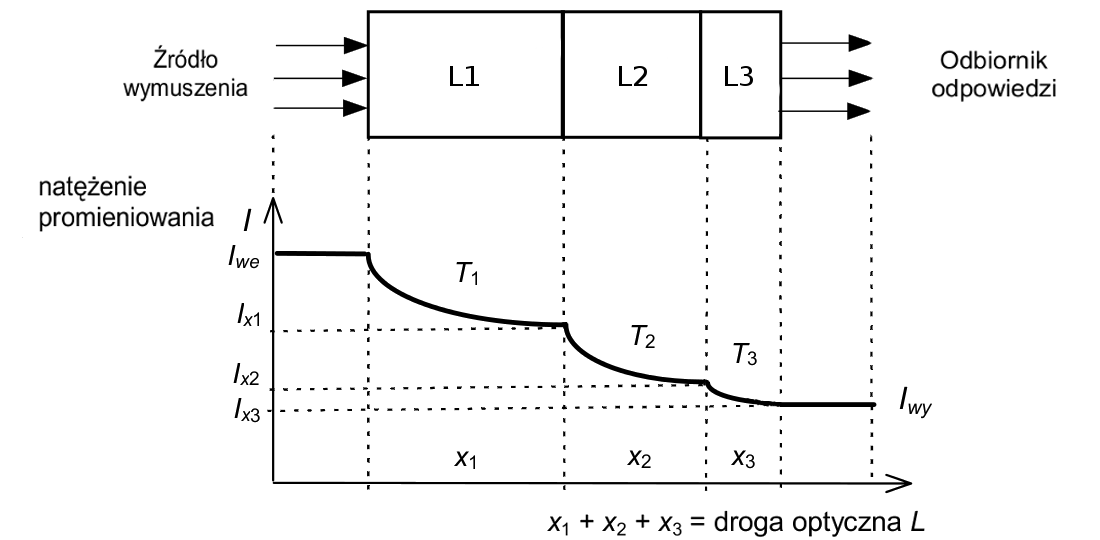
\includegraphics[scale = 0.40]{graphic/multilayer.png}}
	\caption{Absorpcja promieniowania przechodzącego przez ośrodek złożony}
	~\\
	(źródło: Na podstawie \cite{Cys:2007})
	\label{rys:multilayer}
\end{figure}\\

\noindent W~przypadku ośrodka homogenicznego dla $i$ różnych substancji o~odmiennych właściwościach optycznych całkowita absorbancja wynosi:
\begin{equation}
	A=(c_{1}\alpha_{1}(\lambda) + c_{2}\alpha_{2}(\lambda) + ... + c_{i}\alpha_{i}(\lambda))x = (\sum_{i=1}^{n}c_{i}\alpha_{i}(\lambda))x\\
	\label{equ:multilayer3}
\end{equation}
Korzystając z~równania~(\ref{equ:multilayer1}) i~(\ref{equ:multilayer3}), prawo Lamberta-Beera pozwala określić stężenia $n$ różnych substancji absorbujących 
w~homogenicznym środowisku, jeśli absorpcja światła jest mierzona dla $n$ różnych długości fali przy znanych współczynnikach absorbancji molowej 
$\alpha_{i}(\lambda)$~\cite{Katja:2011}.

\section{Rozpraszanie}
\label{sec:Rozpraszanie}
%---------------------------------------------------------------------------

Nazwą tą określa się zjawisko oddziaływania światła z~materią, w~wyniku którego następuje zmiana kierunku rozchodzenia się promieniowania, z~wyjątkiem zjawisk opisanych 
przez odbicie i~załamanie. Rozpraszanie wywołuje złudzenie świecenia ośrodka pod wpływem oddziaływania z~promieniowaniem elektromagnetycznym z~zakresu fal widzialnych~(rys.~\ref{rys:scattering}). 
\begin{figure}[ht]
	\centerline{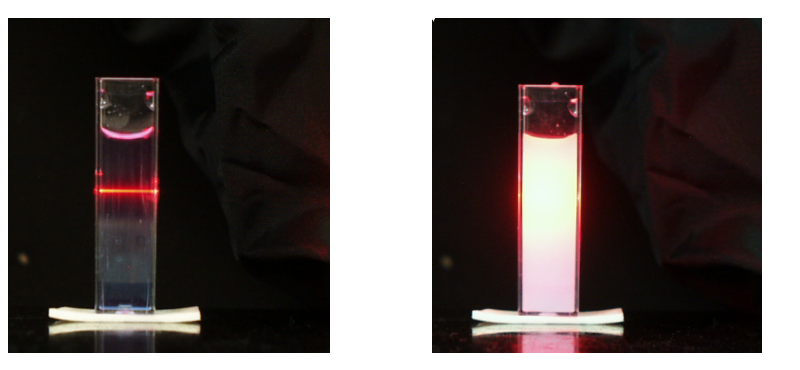
\includegraphics[scale = 0.45]{graphic/scattering.png}}
	\caption{Interakcja promieniowania świetlnego z~materią w~ośrodku nierozpraszającym i~rozpraszającym}
	~\\
	(źródło: Na podstawie \cite{Dwyer:2008})
	\label{rys:scattering}
\end{figure}

\noindent Rozróżnia się następujące jego rodzaje~\cite{Zee:1992}:
\begin{itemize}
	\item sprężyste – podczas rozpraszania nie następuje zmiana energii światła,
	\item niesprężyste – następuje zmiana energii promieniowania w~wyniku rozproszenia.
\end{itemize}

Zjawisko rozpraszania światła można podzielić na trzy rodzaje interakcji światło-cząstka: rozpraszanie Rayleigha, rozpraszanie Mie oraz rozpraszanie Ramana~\cite{Nui:2007}. 
Zjawisko Rayleigha zachodzi przy długości fali $\lambda$ znacznie większej niż wymiary cząstek ośrodka, gdzie rozpraszanie Mie 
występuje przy wymiarach porównywalnych. Zarówno rozpraszanie Rayleigha, jak i~rozpraszanie Mie są sprężyste i~powodują zmianę tylko trajektorii rozproszonego 
fotonu. Teoria Ramana natomiast opisuje zjawisko, w~którym trajektoria rozproszonego fotonu ulega zmianie, ale dodatkowo powoduje emisję światła, zwykle o~większej 
długości fali~\cite{Nui:2007}.

\subsection{Zmodyfikowane prawo Lamberta-Beera dla rozpraszania}
\label{subsec:LBrozpraszanie} 

Poprzez analogię do zjawiska absorpcji promieniowania, efekt rozpraszania fotonów wewnątrz medium transmisyjnego również wprowadza osłabienie wiązki w~kierunku 
propagacji fali elektromagnetycznej. Współczynnik $\mu_{s}$ opisuje stratę natężenia promieniowania na skutek rozproszenia, co wspólnie ze zjawiskiem absorpcji 
zapisuje się następująco:

\begin{equation}
	I(x) = Ie^{-\mu_{t}x}
\end{equation}
dla
\begin{equation}
	\mu_{t} = \mu_{a} + \mu_{s}
\end{equation}
gdzie:\\
$\mu_{a}$ - współczynnik absorpcji promieniowania,\\
$\mu_{s}$ - współczynnik rozpraszania promieniowania.\\

W~tkankach biologicznych dominujący wpływ mają zjawiska opisane przez Rayleigha oraz Mie~\cite{Nui:2007}, których podstawową różnicą jest odmienna kierunkowość 
natężenia promieniowania wtórnego~(rys.~\ref{rys:scattering_3}). Rozkład kątowy intensywności światła rozproszonego dla zjawiska Rayleigha jest osiowo symetryczny 
względem linii przechodzącej przez elementarną cząstkę rozpraszającą w~kierunku propagacji fali padającej. Maksymalne rozpraszanie występuje w~płaszczyźnie równoległej 
do kierunku wiązki padającej~(rys.~\ref{rys:scattering_3}a). Rozpraszanie Mie charakteryzuje silna zależność rozkładu intensywności od kierunku. Obserwuje się asymetrię 
między rozpraszaniem w~przód i~w~tył: przeważa rozpraszanie w~przód~(rys.~\ref{rys:scattering_3}b).
\begin{figure}[!ht]
	\centerline{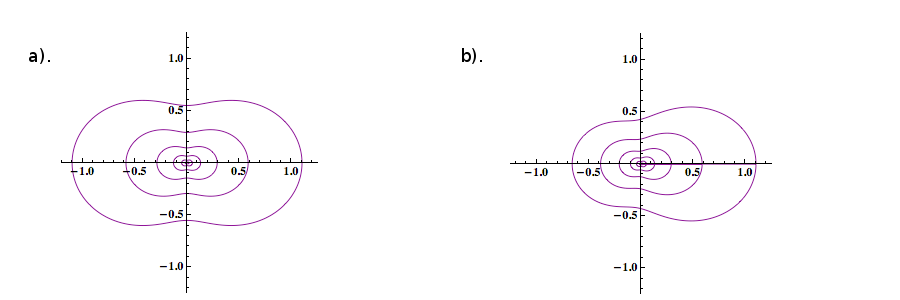
\includegraphics[scale = 0.62]{graphic/scattering_3.png}}
	\caption{Zależność rozkładu intensywności promieniowania rozproszonego od kierunku propagacji dla zjawiska Rayleigha~(a) oraz Mie~(b)}
	~\\
	(źródło: http://pages.vassar.edu)
	\label{rys:scattering_3}
\end{figure}

\subsection{Funkcja fazowa i~współczynnik anizotropii}
\label{subsec:PhaseAnisotropy}

Rozpraszanie promieniowania w~tkankach nie jest zjawiskiem izotropowym~\cite{Yavari:PhD:2006}. Natężenie promieniowania emitowanego jest zmienne w~zależności 
od kąta odchylenia od kierunku propagacji.

Należy zdefiniować funkcję fazową $p(\theta)$ wyznaczającą prawdopodobieństwo $p$ rozproszenia kwantu promieniowania pod danym kątem $\theta$. Prawdopodobieństwo 
rozproszenia fotonu zależy wyłącznie od wyboru kąta odchylenia pomiędzy wektorem jednostkowym rozproszenia $\hat{s}'$ a~wektorem zgodnym z~kierunkiem propagacji fali 
padającej $\hat{s}$:
\begin{equation}
	p(\theta)=p(\hat{s}', \hat{s})
\end{equation}
Funkcja fazowa $p(\theta)$ Henyeya-Greensteina~(\ref{equ:HenyeyGreenstein}) jest stosowana podczas analizy zjawiska rozpraszania w~ośrodkach złożonych z~tkanek 
biologicznych~\cite{Yavari:PhD:2006}. 

\begin{equation}
	p(\theta)=\frac{1}{4\pi}\frac{1-g^2}{(1+g^2-2gcos(\theta))^{\frac{3}{2}}}
	\label{equ:HenyeyGreenstein}
\end{equation}
gdzie spełniona jest zależność:

\begin{equation}
	\int_{0}^{\pi} p(\theta)2\pi sin(\theta)d\theta=1
\end{equation}
Parametr $g$ opisuje stopień anizotropii rozpraszania promieniowania w~ośrodku.
Wpływ współczynnika anizotropii na charakterystykę kierunkową rozpraszania przedstawiono na rysunku \ref{rys:anisotropy}. Zakres 
wartości parametru $g$~zawiera się w~zakresie od -1~(całkowite rozpraszanie w~tył) do wartości 1~(całkowite rozpraszanie w~przód).
Dla $g=0$ rozpraszanie ma charakter izotropowy. 

\subsection{Zredukowany współczynnik rozpraszania}
\label{subsec:ReducedFactor}

Wyrażenie na współczynnik efektywnego rozpraszania w~ośrodku rozpraszającym powinno uwzględniać zarówno współczynnik rozpraszania $\mu_{s}$,
jak i~współczynnik anizotropii~$g$. 
\noindent Zredukowany współczynnik rozpraszania $\mu_{s}'$ łączy wspomniane parametry w~następujący sposób:
\begin{equation}
	\mu_{s}'=\mu_{s}(1-g)
	\label{equ:reduced_mu}
\end{equation}
\begin{figure}[ht]
	\centerline{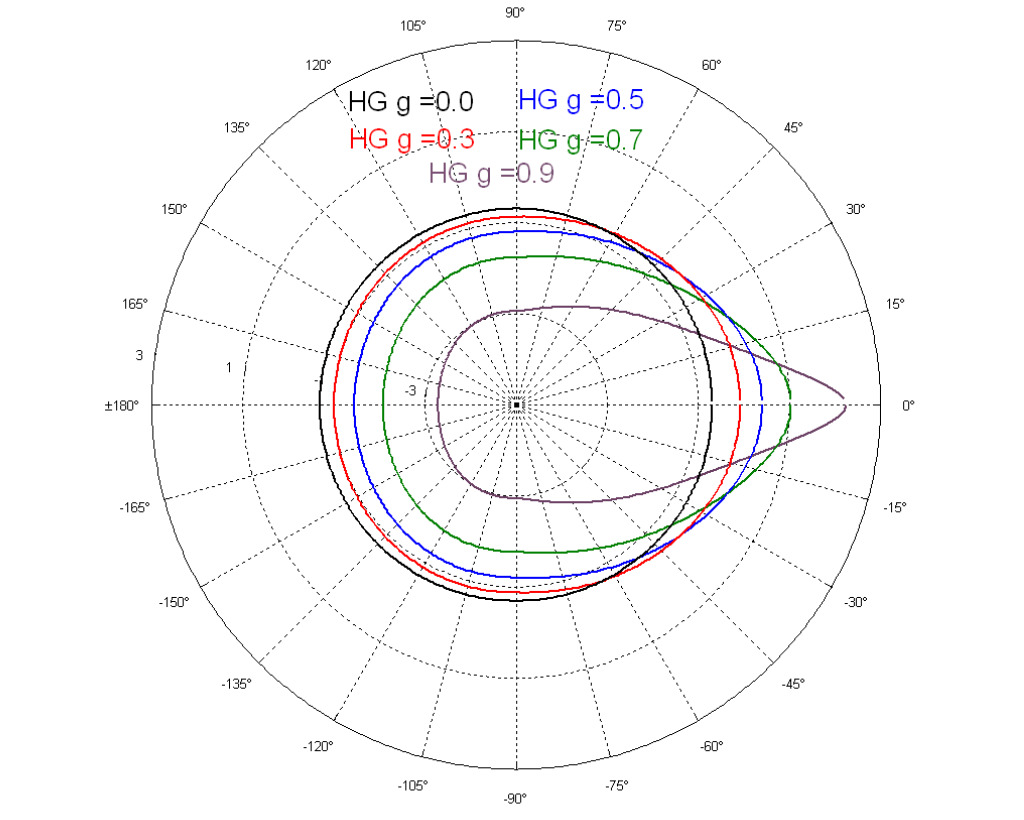
\includegraphics[scale = 0.45]{graphic/HenyeyGreenstein.png}}
	\caption{Przebieg funkcji Henyeya-Greensteina dla wybranych wartości współczynnika anizotropii $g$}
	~\\
	(źródło: http://openi.nlm.nih.gov)
	\label{rys:anisotropy}
\end{figure}

\noindent Całkowity współczynnik tłumienia promieniowania wewnątrz ośrodka rozpraszającego i~absorbującego po uwzględnieniu współczynnika anizotropii przedstawia
się następująco:
\begin{equation}
	\mu_{t}'=\mu_{a} + \mu_{s}'
\end{equation}

